% コピペスタート
\documentclass[8pt, jfont=ipaexm, t]{beamer} % IPAex明朝
\usepackage{hyperref}
% 一般的によく使用されるパッケージ
\usepackage{caption}
\usepackage[utf8]{inputenc}
\usepackage{graphicx}
\usepackage{amsmath}
\usepackage{amsfonts}
\usepackage{amssymb}
\usepackage{tikz}
\usepackage{pgfplots}
\pgfplotsset{compat=1.18}   % pgfplots のバージョンを指定
\usepackage{listings}
\usepackage{array}

% スタイル設定
\usepackage{ifthen}
\usepackage[varg]{txfonts}
\usepackage{ragged2e}
\usepackage{svg}
\usepackage{xcolor}
\usepackage{url}
\usepackage{bm}

\usetikzlibrary{graphs}
\usetikzlibrary {arrows.meta}
\usetikzlibrary {bending}
\usetikzlibrary{arrows,shapes,automata,petri,positioning,calc}


% 和文用パッケージ(luatex用)
\usepackage{luatexja}
% \usepackage{luatexja-fontspec}
\usepackage{lmodern}
\usepackage[T1]{fontenc} % 必要に応じてフォントエンコーディングを指定


%カラーテーマの選択(省略可)
\usecolortheme{orchid}
%フォントテーマの選択(省略可)
\usefonttheme{professionalfonts}
%フレーム内のテーマの選択(省略可)
\useinnertheme{circles}
%フレーム外側のテーマの選択(省略可)
\useoutertheme{infolines}
%しおりの文字化け解消
% \AtBeginShipoutFirst{\special{pdf:tounicode EUC-UCS2}}

% \AtBeginShipoutFirst{\special{pdf:tounicode 90ms-RKSJ-UCS2}}
%ナビゲーションバー非表示
\setbeamertemplate{navigation symbols}{}

% タイトル色
\setbeamercolor{title}{fg=structure, bg=}

% フレームタイトル色
\setbeamercolor{frametitle}{fg=structure, bg=}

% caption に番号追加
\setbeamertemplate{caption}[numbered]
% caption 日本語
\renewcommand{\figurename}{図}
\renewcommand{\tablename}{表}

\usepackage[export]{adjustbox} % loads also graphicx


\usetheme[progressbar=frametitle, block=fill, numbering=fraction,]{metropolis}
% \usetheme{default}
            
% ブロックのスタイルをカスタマイズ
\setbeamertemplate{blocks}[rounded]
\setbeamercolor{block title}{bg=gray!30,fg=black} % ブロックのタイトルの背景とフォントの色
\setbeamercolor{block body}{bg=gray!10,fg=black} % ブロック本体の背景とフォントの色

\setbeamercolor{block title example}{bg=orange!30,fg=black} % 例のブロックのタイトルの背景とフォントの色
\setbeamercolor{block body example}{bg=orange!10,fg=black} % 例のブロック本体の背景とフォントの色

\setbeamercolor{block title alerted}{bg=red!30,fg=black} % アラートのブロックのタイトルの背景とフォントの色
\setbeamercolor{block body alerted}{bg=red!10,fg=black} % アラートのブロック本体の背景とフォントの色

\tikzset{set label/.style={fill=white,circle,inner sep=2}}

\def\radius{2}
\def\ratio{0.6}

\def\centerA{180:\ratio*\radius}
\def\circleA{(\centerA) circle [radius=\radius]}





%追加
\setbeamertemplate{footline}{%
  \hfill%
  \usebeamercolor[fg]{page number in head/foot}%
  \usebeamerfont{page number in head/foot}%
  \insertframenumber\,/\,\inserttotalframenumber\kern1em\vskip2pt%
}

%ソースコードに関する設定
\lstset{
    language={C++}, 
    basicstyle={\ttfamily},
    identifierstyle={\small},
    commentstyle={\smallitshape},
    keywordstyle={\small\bfseries},
    ndkeywordstyle={\small},
    stringstyle={\small\ttfamily},
    frame={tb},
    breaklines=true,
    columns=[l]{fullflexible},
    numbers=left,
    xrightmargin=0em,
    xleftmargin=3em,
    numberstyle={\scriptsize},
    stepnumber=1,
    numbersep=1em,
    lineskip=-0.5ex
}


\tikzset{
    place/.style={
        circle,
        thick,
        draw=black,
        fill=gray!50,
        minimum size=6mm,
    },
        state/.style={
        circle,
        thick,
        draw=blue!75,
        fill=blue!20,
        minimum size=6mm,
    },
}

\title{計算量について}
\author{佐藤謙成}
\institute{KUT-PG}

\begin{document}
\begin{frame}
    \titlepage
\end{frame}

\begin{frame}{目次}
    \tableofcontents[]
\end{frame}


\section{計算量(オーダー)}
\begin{frame}{オーダー記法}
    \begin{block}{オーダー記法とは}
        アルゴリズムの計算量を評価するための記法. $t$ を時間とすると,$O(t)$で表すことができる. $t$は小さい方が計算量が少ないため,評価は高くなる.
        \begin{itemize}
            \item アルゴリズムによって所要時間が異なる
            \item 良いアルゴリズムの場合は解決したい問題の規模が大きくなっても対抗可能である.
        \end{itemize}
        
        以下は, $t$に入る代表格である.
        \begin{align*}
            \log{n} < \sqrt{n} < n < n\log{n} < n^2 < n^3 < \cdots < 2^n < n!
        \end{align*}
        できるだけ $\log{n} $になるようにアルゴリズムを組んでいきたい.
    \end{block}
    
    \begin{block}{オーダー記法($t$)の決め方}
        \begin{enumerate}
            \item アルゴリズムの時間計算量を入力サイズ $n$ を用いた関数で表す.
            \item その関数の中で主要項\footnote{$n$ が一番大きいもの}を見つける.
            \item 主要項の係数を削除した関数が $f(n)$である時,アルゴリズムの時間計算量は $O(f(n))$であるという.
        \end{enumerate}
    \end{block}
\end{frame}

\begin{frame}{実行時間}
    アルゴリズムの実行時間に関して,以下の語句で表現される.
    \begin{enumerate}
        \item 時間計算量
        \item 最良時間計算量
        \item 最悪時間計算量
        \item 領域計算量
        \item 平均時間計算量
    \end{enumerate}
    \begin{block}{最良時間計算量}
        最も速くそのアルゴリズムを実行できる入力の時間計算量.
    \end{block}
    \begin{block}{最悪時間計算量}
        最も時間のかかる入力に対する時間計算量. .
    \end{block}
    \begin{block}{平均時間計算量}
        入力データがランダムに分布している場合の計算時間を示す.
    \end{block}
    \begin{block}{領域計算量}
        アルゴリズムを実行する際にどれだけのメモリ(領域)が必要かを表す.
    \end{block}
\end{frame}

\begin{frame}{計算量の評価}
\begin{block}{}
計算量の評価は以下の通りとなる.
    \begin{align*}
    \log{n} < \sqrt{n} < n < n\log{n} < n^2 < n^3 < \cdots < 2^n < n!
    \end{align*}
\end{block}
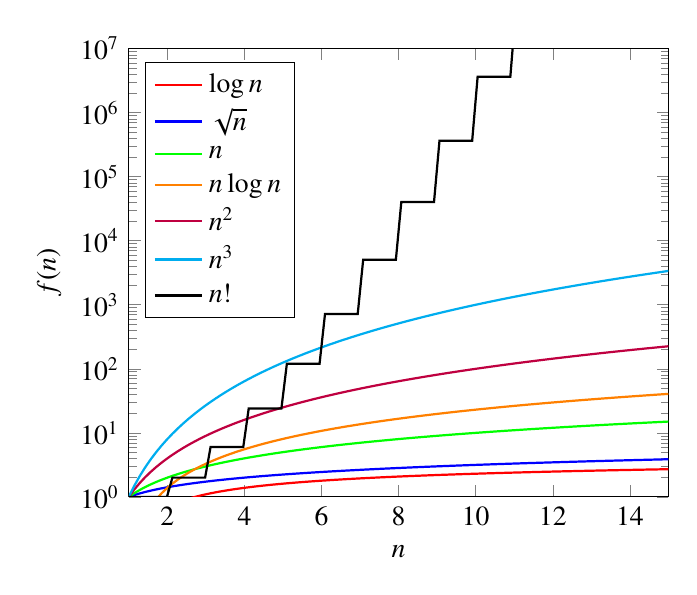
\begin{tikzpicture}
    \begin{axis}[
        xlabel={$n$},
        ylabel={$f(n)$},
        legend pos=north west,
        ymode=log,                % y軸に対数スケールを使用
        xmin=1, xmax=15,          % X軸の範囲(表示用)
        ymin=1, ymax=1e7,         % Y軸の範囲(表示用)、n! のために ymax を増加
        samples=100,              % プロット用のサンプル数
        domain=1:15,              % xの計算ドメイン(nの値は1から10)
        legend cell align={left}, % 凡例の項目を左揃えにする
        % grid=both,              % グリッドが必要な場合はコメントを外す
    ]
    \addplot[thick, color=red]   {ln(x)};        \addlegendentry{$\log{n}$}
    \addplot[thick, color=blue]  {sqrt(x)};      \addlegendentry{$\sqrt{n}$}
    \addplot[thick, color=green] {x};            \addlegendentry{$n$}
    \addplot[thick, color=orange]{x*ln(x)};      \addlegendentry{$n\log{n}$}
    \addplot[thick, color=purple]{x^2};          \addlegendentry{$n^2$}
    \addplot[thick, color=cyan]  {x^3};          \addlegendentry{$n^3$}
    \addplot[thick, color=black]  {x!};       \addlegendentry{$n!$}
    \end{axis}
\end{tikzpicture}
\end{frame}

\begin{frame}{基本演算での時間計算量}
\begin{block}{}
        \begin{itemize}
        \item 算術演算
        \item 論理演算
        \item 入出力の命令
    \end{itemize}
    これらの基本演算の時間計算量は $O(1)$(定数時間)となる.
\end{block}
\end{frame}

\begin{frame}{時間計算量の例.1}
    以下のアルゴリズムの時間計算量を求めていく.
    \begin{exampleblock}{アルゴリズムA}
        $10n^2 + 100n + 10000$
    \end{exampleblock}
    \begin{exampleblock}{アルゴリズムB}
        $n^4 - n^3 + 100$
    \end{exampleblock}

        \begin{block}{再掲}
        \begin{enumerate}
            \item アルゴリズムの時間計算量を入力サイズ $n$ を用いた関数で表す.
            \item その関数の中で主要項\footnote{$n$ が一番大きいもの}を見つける.
            \item 主要項の係数を削除した関数が $f(n)$である時,アルゴリズムの時間計算量は $O(f(n))$であるという.
        \end{enumerate}
    \end{block}
\end{frame}

\begin{frame}[fragile]{時間計算量の例.2}
以下のコードを元に時間計算量を求めていきたい.(計算量オーダーは,最悪時間計算量について考えるのが基本である.)
    \lstinputlisting{./code/order/for.txt}
\begin{exampleblock}{}
    \begin{itemize}
        \item if文の時間計算量は, $O(1)$である.
        \item 外側のfor文の繰り返し回数は, $n - 1$回.
        \item 内側のfor文の繰り返し回数は, $n - i$回.
    \end{itemize}
    このアルゴリズムの時間計算量は,
    \begin{align*}
        O(1) \times \dfrac{n(n - 1)}{2} = O(n^2)
    \end{align*}
\end{exampleblock}
\end{frame}

\begin{frame}{計算量の使い方}
    実際の問題をに対してアルゴリズムを設計する時の考え方について考えていく.
    
    通常の計算機では 1 秒間に処理できるfor文のループの回数は, $ 10^8 $ 回程度である.
    (Atcoderでは通常,制限時間が2秒間であるので命令実行の回数は $2 \times 10^8$ 回程度である.)
    \[
        \begin{array}{ *{7}{l}}
        \log{n} & n & n\log{n} & n^2 & n^3 & 2^n & n! \\
        \hline
        2 & 5 & 12 & 25 & 130 & 30 & 120 \\
        3 & 10 & 33 & 100 & 1000 & 1024 & 362880 \\
        4 & 15 & 59 & 225 & 3375 & 32768 & - \\
        4 & 20 & 86 & 400 & 8000 & 1048576 & - \\
        5 & 25 & 116 & 625 & 15625 & - & - \\
        5 & 30 & 147 & 900 & 27000 & - & - \\
        7 & 100 & 664 & 10000 & 1000000 & - & -
        \end{array}
    \]
\end{frame}
\end{document}
